\chapter{Problem Statement}
\label{cha:multiObjectiveOptimization}



%---------------------------------------------------------------------------

\section{Multi-objective optimization}
\label{sec:multi}

The main goal of optimization is to find the very best solution from a most likely infinite set of possibilities.
Optimization procedure relies on finding and comparing feasible solutions until no better solution can be found.
Each solution can be classified as good or bad in terms of a specific objective we are interested in.
E.g. we could define objective as the cost of fabrication, efficiency of a technological process, etc.
Contrary to single-objective optimization there is no clearly defined optimum, instead of that we have to deal with a set of trade-off optimal solutions.
They are generally known as Pareto-optimal solutions \cite{Phd}.

Vast majority of real-world problems involve more than one objective.
That's why it is so crucial to develop methods to efficiently solve them 
\cite{Phd}, \cite{Deb:2001:MOU:559152}.

\subsection{Formal definition}

Multi-objective optimization problem (MOOP) deals with more than one objective function.
It turns out that objectives are most likely contradictory which makes the MOOP difficult to solve.
In fact it is the most common situation we will ever encounter. 
Following \cite{Deb:2001:MOU:559152} - formal definition of MOOP is being defined as follows:

\begin{equation} 
MOOP \equiv
 \begin{cases}
     Minimize/Maximize  & f_{m}(\bar{x}), \text{ } m = 1,2...,M \\
     Subject \text{ } to  &  g_{j}(\bar{x}) \geq 0, \text{ } j = 1,2..., J  \\ 
			  &  h_{k}(\bar{x}) = 0, k = 0,1...,K \\
			  &  x_{i}^{(L)} \leq x_{i} \leq x_{i}^{(U)}, i = 1,2...,N
      
\end{cases}  
\end{equation}

These constraints and bounds ($g_{j}(x) , h_{k}(x) $ are constraint functions and there are $M$ objective functions) constitute a \emph{decision space}  
\cite{Deb:2001:MOU:559152}.
Any solution that satisfies all the constraints and bounds is called a \emph{feasible solution} \cite{Deb:2001:MOU:559152}.

It turns out that the set of feasible solutions is partially ordered.
In order to compare two solutions we introduce \emph{Pareto dominance} relation \cite{Phd}:

\begin{equation}
\bar{x}_{A}  \prec \bar{x}_{B} \equiv
      \begin{cases}
     \exists{i \in 1..M} : f_{i}(\bar{x}_{A}) < f_{i}(\bar{x}_{B}) \\
     \neg (\exists{j \in 1..M} : f_{j}(\bar{x}_{A}) > f_{j}(\bar{x}_{B}))  \\ 
			  
      
\end{cases} 
\end{equation}

Solution that is not dominated by any other solution is called \emph{non-dominated}. 
The set of \emph{non-dominated} solutions is what we are actually trying to find while dealing with MOOPs.



\begin{figure}[ht]
  \begin{center}
    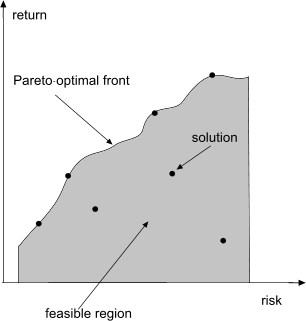
\includegraphics[scale=.9]{pareto_front.png}
  \end{center}
  \caption{Pareto-optimal front of portfolio optimization problem}
\end{figure}


Pareto-optimal front is the set of choices that are \emph{non-dominated} (\cite{Dre}).
 

\subsection{Portfolio optimization problem}

First of all, let us introduce the definition of \emph{portfolio}.
	\emph{Portfolio} is a set of assets or equities (e.g. stocks, bonds) owned by an investor.
	Usually the more diversified the  \emph{portfolio} the safer our investments tend to be.
	\emph{Portfolio} composition should reflect our willingness to take risk.

Portfolio optimization problem is an example of MOOP.
Investors cannot rely solely on their intuition to make the right choice.
It is obvious that every investor would like to have the highest return possible.
Unfortunately, equities with high returns usually correlate with high risk. 
That is why it is up to the investor to decide what level of risk is acceptable.

%---------------------------------------------------------------------------

\section{Capital Asset Pricing Model}
\label{CAPM}

%\cite{CAPM}

Modern Portfolio Theory (MPT) (introduced by Harry Markowitz in 1952) was a tremendous breakthrough. 
Investors could finally use a mathemathical approach to construct their portfolios.
Most of them used solely diversification as a mean of reducing portfolio risk.
With brand new theory they did not have to rely only on common sense - the investment risk was finally expressed in quantitative terms. 

Nevertheless MPT is not perfect, even its creators are fully aware that it has some very important limitations.
The following assumptions of MPT are responsible for its shortcomings \cite{MPT}, such as:
\begin{itemize}
  \item variance of portfolio returns is the correct measure of investment risk;
  \item investment returns of all assets can be adequately represented by the normal distribution.
\end{itemize}

  

Capital Asset Pricing Model (CAPM) was developed in 1960s by Sharpe (\cite{CAPM-Sharpe}) and Lintner.
 
As well as MPT it tries to find the relationship between the price of a single asset and its risk.
Answering the question of how to calculate a risk as well as return of any asset being a part of portfolio is of great importance to each investor.

The Sharpe capital asset pricing model is based on the following assumptions \cite{CAPM}:

\begin{itemize}
  \item all investors are risk aversing;
  \item all investors have the same information about the market;
  \item capital markets are perfect - no transaction costs, no tax, all assets are infinitely divisible;
  \item all investors view the expected returns and standard deviations of return provided by different portfolios in the same way.
\end{itemize}
 
In order to fully understand CAPM, we have to introduce some definitions.

First of all, we define $population$ (statistics) as a set containing all entities that are relevant in a statistical study of a particular problem \cite{Oxford}.
The concept of $population$ is crucial to define the rest of definitions that are used.

$Population$ $mean$ is the mean of an observation variable is a numerical measure of the central location of the data values.
	The $population$ $mean$ is defined as:
	 \begin{equation}
			\mu = \frac{1}{N} \sum_{i=1}^{N}{(x_{i})} 
		      \end{equation}

The next important function is $population$ $variance$, it is a numerical measure of how the data values is dispersed around the mean.
	The $population$ $variance$ is defined as:  
	      \begin{equation}
			\sigma^2 = \frac{1}{N} \sum_{i=1}^{N}{(x_{i} - \mu)} 
		      \end{equation}
	where $\mu$ is a population mean.

The $standard$ $deviation$ of a population ($\sigma$) is defined as a square root of the population variance.
	
The $covariance$ of two variables $x$ and $y$ in a data sample measures how the two are linearly related.
	A positive $covariance$ would indicate a positive linear relationship between the variables, and a negative $covariance$ would indicate the opposite. 
	The population $covariance$ is defined as:

	\begin{equation}
			\sigma_{xy} = \frac{1}{N} \sum_{i=1}^{N}{(x_{i} - \mu_{x})(y_{i} - \mu_{y})} 
		      \end{equation}
	where $\mu_{x}$ and $\mu_{y}$ are population means.

Last but not least, we introduce $correlation$ $coefficient$ as a normalized measurement of how the two variables in a data sample are linearly related.
	The population $correlation$ $coefficient$ is defined as:

	\begin{equation}
	  \rho_{xy} = \frac{\sigma_{xy}}{\sigma_{x} \sigma_{y}}
	\end{equation}
	where $\sigma_{x}$ and $\sigma_{y}$ are the population standard deviations and $\sigma_{xy}$ is the population covariance.
	

Now we are ready to finally give formulas for expected return and risk.

Lets assume that investor portfolio contains $N$ assets, then according to Capital Asset Pricing expected return of asset $i$ is \cite{CAPM}: 

\begin{equation}
\label{first_eq}
 E(R_{i})  = R_{f} + \frac{ [E(R_{m}) - R_{f}]} {\sigma^2(R_{m})} cov(R_{i}, R_{m})
\end{equation} 

where:
\begin{description}
  \item [$E(R_{i})$]
    - expected return of asset $i$;
  \item [$R_{f}$]
    - risk-free rate of interest (e.g. government bonds);
  \item [$E(R_{m})$]
    - expected return of the market;
  \item [$\sigma^2(R_{m})$]
    - variance of the market return;
  \item [$cov(R_{i}, R_{m})$]
    - covariance between market return and asset $i$ return.
\end{description}

While the risk associated with entire portfolio is equal to:

\begin{equation}
\label{sec_eq}
 \sigma_{p}  = \sqrt{\sum_{i} \sum_{j} w_{i}w_{j} \sigma_{i} \sigma_{j} \rho_{ij}}
\end{equation} 

where:

\begin{description}
  \item [$\sigma_{p}$]
    - portfolio risk;
  \item [$w_{i}$]
    - weighting of component asset $i$;
  \item [$w_{j}$]
    - weighting of component asset $j$;
  \item [$\sigma_{i}$]
    - standard deviation of asset $i$;
  \item [$\sigma_{j}$]
    - standard deviation of asset $j$;
  \item [$\rho_{ij}$]
    - correlation coefficient between the returns on assets $i$ and $j$.
\end{description}
 
%---------------------------------------------------------------------------

\section{Trend following}
\label{sec:trendFollowing}

\subsection{Trend following fundamentals}
\label{sec:trend_following_fundamentals}

The concept of price as the trading cue lays the foundations for trend following (TF). 
Contrary to other trading strategies based on fundamental analysis (which use factors like: overall state of the economy, interest rates, production, etc. to predict stock price)
TF use only price as the key trading variable. 

Trend following basically does not try to predict when the trend will occur. 
Instead of that, trend followers will react to the market's movement and adapt accordingly.
This strategy simply analyses stock prices and decides whether the current situation is suitable for buying or selling a specific stock.
Market breakouts are a great buying opportunities, on the other hand when you recognize that you are wrong you exit immediately in order to cut losses.
Set of predefined rules decides  whether to take any action (they should recognize when the trend starts as well as when to exit) so the entire process can be easily automated.
Such rules are quite simple but disciplined execution of them could lead to achieving spectacular returns year after year.
It is all about cutting the losses and letting the profits run.
Many leading hedge funds successfully use strategies based on trend following to manage their portfolios \cite{Trend01}.  

\begin{figure}[ht]
  \begin{center}
    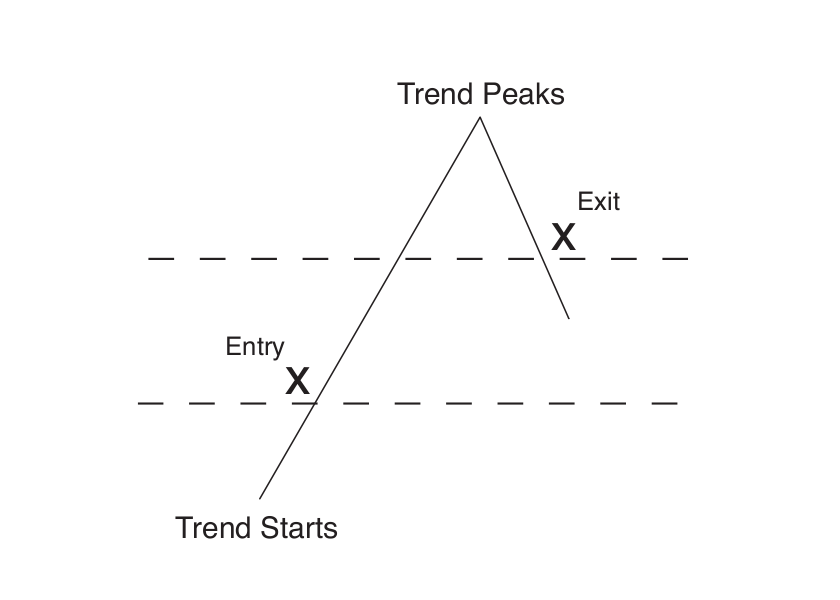
\includegraphics[scale=.4]{trend_following.png}
  \end{center}
  \caption{Simple example of how trend following works in practise (\cite{Trend01})}
\end{figure}

Another advantage of this investing method is the fact that investor does not have to know much about what is being traded (it could be stocks, oil, gold, etc.).
Normally, people tend to gather some information about the company they are willing to invest in. 
They analyse its market situation, competitors, financial performance, etc. which is time consuming, especially for someone who is not a professional trader.
With trend following we just have to focus on elaborating trading rules that should reflect our trading strategy.
After that, we can automate the decision making process by designing and implementing our own trading system.   

\subsection{Types of trends}
\label{sec:types_of_trends}

There are three main types of trends:

\begin{enumerate}
  \item \textbf{Short-term trend}: any price movement that occurs over a few hours or days.
  \item \textbf{Intermediate-term trend}: general movement in price data that lasts from three weeks to six months.
  \item \textbf{Long-term trend}: any price movement that occurs over a significant period of time, often over one year or several years.
\end{enumerate}



\subsection{Designing trading system based on trend following} 

Following \cite{Trend01}, the core of each trading system based on trend following strategy is a set of rules governing each buy/sell decision.
More specifically we have to devise rules to answer the following questions:

\begin{itemize}
  \item how much money are we willing to put on a single trade;
  \item when to exit (what kind of losses are acceptable);
  \item when to enter (when the trend has started); 
  \item what markets are we interested in and how to split money between them (we would like to have a diverse portfolio (stocks, gold, etc.)).
\end{itemize}

These rules should reflect our investing style.

In \ref{trend_following_impl} a system based on trend following strategy is presented in more details.

%---------------------------------------------------------------------------

\section{Evolutionary algorithms}
\label{sec:evolAlgorithms}

Darwin's theory of evolution introduces the concept of survival of the fittest - in environments with limited resources individuals have to compete for them and
only the best adapted to environmental conditions survive.
Each individual has a set of traits that determine its fitness.
The fitter the individual the more likely its genetic information will be further propagated.
Darwin observed that small random changes in genotype (mutations), which introduce completely new traits, could be beneficial to an individual.
In that case, they would most likely be inherited by its children \cite{evo}.


Each stochastic optimization method based on a simulation of evolution process (natural evolution is simulated by an iterative computation process)
can be termed as the Evolutionary Algorithm (EA).
Most commonly known examples of EA include genetic algorithms and evolutionary programming.
A set of candidate solutions, which is modified by the principles of evolution (selection and variation), is used by all above approaches.
Some of solutions present in the population set are better than others (we can assign a fitness value to each solution).
The fitter the solution the more likely it will reproduce.
By means of recombination and mutation new chromosomes are introduced into existing population.
Despite the fact that the principles are quite simple, the resulting algorithm is a powerful search mechanism.  

Apart from all advantages mentioned above, evolutionary algorithms are especially usefull to solve \emph{Multi Objective Optimization Problems} because they
can find multiple \emph{non-dominated} solutions at once. 
According to some researchers evolutionary algorithms are much better suited for MOOPs than strategies based on blind search \cite{Phd}.

\subsection{Basic principles of evolutionary algorithms}

Following \cite{Phd}, EA can be characterized by:

\begin{itemize}
  \item set of possible solutions is kept throughout the algorithm execution;
  \item selection process (low quality individuals are removed while well fitted are allowed to reproduce);
  \item set of possible solutions is manipulated by genetic operators (e.g. mutation and recombination).
\end{itemize}

Solution candidates are usually called \emph{individuals} and the entire set of them is called a \emph{population}. 
Fitness function (evaluation function) has one main role - it is responsible for assessing individuals, thus it defines what does it mean to be fit in a particular
environment.

There are theorems stating that an evolutionary algorithm will reach a global optimum of a particular problem if we can guarantee that every genotype representing
potential solution can be obtained by the application of genetic operators.
Mutation can be used to asure that property, as it is introducing random changes to a solution, thus allowing us to literally jump into parts of the solution space
that we would not discover \cite{evo}.       

Recombination simply merges the genetic information of both parents in order to produce offspring.
The merging operation depends on random values, therefore the whole process is stochastic.
Because we are merging two individuals with good traits we hope to get similarly well adjusted individual.
That strategy is a base for animal husbandry used since ancient times.
   
Obviously evolutionary algorithms resemble other general algorithm construction techniques like greedy algorithms (at each step we choose locally optimal decision, which 
turns out to be globally optimal) or dynamic programming (thanks to remembering results of some of the subresults we are able to solve some problems 
in polynomial time, but often with additional memory needed).
All of them have to be adjusted to actually solve our problem.
Greedy approach is certainly the simplest and most straightforward but we have to be careful because many problems do not have $optimal$ $substructure$ (optimal solution
to problem contains optimal solution to sub-problem).
If our optimisation problem does not have that property we may end up with completely wrong solution.
Dynamic programming demands $optimal$ $substructure$ from problems as well.
It is a much more complicated way of contructing algorithms and some problems are really hard to adapt to that method.
 

\subsection{Pseudocode of an evolutionary algorithm}

Following \cite{evo}, the general scheme of evolutionary algorithm is presented in Algotithm~\ref{pseudo_EA}.
 
% \begin{algorithmic}
% 
% \STATE INITIALISE $population$ with random candidate solutions
% \STATE EVALUATE each candidate
% \REPEAT
%   \STATE SELECT parents
%   \STATE RECOMBINE pairs of parents
%   \STATE MUTATE the resulting offspring
%   \STATE EVALUATE new candidates
%   \STATE SELECT individuals for the next generation
% \UNTIL{TERMINATION CONDITION is satisfied}
% 
% 
% \end{algorithmic}


\begin{algorithm}
  \SetKwData{returnOrientedSubpopulation}{returnOrientedSubpopulation}
  \SetKwData{riskOrientedSubpopulation}{riskOrientedSubpopulation}
  \SetKwData{parents}{parents}
  \SetKwData{offspring}{offspring}
  \SetKwData{population}{population}
  \SetKwData{mutants}{mutants}
  \SetKwFunction{evaluate}{evaluate}
  \SetKwFunction{initialise}{initialise}
  \SetKwFunction{selectParents}{selectParents}
  \SetKwFunction{recombine}{recombine}
  \SetKwFunction{merge}{merge}
  \SetKwFunction{mutate}{mutate}
  \SetKwFunction{select}{select}
  \SetKwInOut{Input}{input}\SetKwInOut{Output}{output}
 
  \BlankLine
  \initialise{\population} \;
  
  \ForEach{$individual$ $\in$ \population}{
	  \evaluate($individual$)\;
  }

  \Repeat{TERMINATION CONDITION is satisfied}{
     
      \parents $\leftarrow$  \selectParents{\population} \;
      \offspring $\leftarrow$ \recombine{\parents} \;
      \mutate{\offspring} \;

      \ForEach{$individual$ $\in$ \offspring}{
	  \evaluate($individual$)\;
      }

      \population $\leftarrow$ \select{\population,\offspring} \;
      
  }
  \caption{Pseudocode of generic EA (\cite{evo})}\label{pseudo_EA}  
\end{algorithm}

We start each round of computation by selecting parents from the entire population.
As mentioned previously, the fitter the individual the more likely it will participate in the process of reproduction.
Mutation is applied to newly created offspring, but with very low probability.
After new individuals evaluation, we have to decide which organisms will survive to next round of computation. 


\subsection{Population diversity}
\label{sec:population_diversity}

Population diversity is essential for finding a large number of Pareto-optimal solutions in a single run of an algorithm.
There are some well established methods of overcoming the problem of premature convergence towards a single solution \cite{Phd}. 

Following \cite{Phd}, the most common methods of maintaining population diversity include:

\begin{enumerate}

  \item \textbf{Fitness sharing}:
	the main idea behind this method is to divide the entire population of individuals into subpopulations.
	Individuals in subpopulations have to share resources.
	If an individual has many close neighbours (in terms of predefined distance measure) its fitness is lower compared to situation when there are
	no other individuals in vicinity. 
	
  \item \textbf{Restricted mating}:
	the gist of this method is to allow two individuals to mate only if they are substantially different (different in terms of some predefined metric).
  \item \textbf{Isolation by distance}:
	the concept of location is introduced so distinct subpopulations can exchange individuals by the process of migration. 
  \item \textbf{Overspecification}:
	apart from solution to the problem, each individual contains unused part of information (which is not taken into consideration during fitness calculation)
	that can manifest itself at some point in the future.
  \item \textbf{Reinitialization}:
	The whole population or at least a significant part is reinitialized after some time or when the search process stagnates.
  \item \textbf{Crowding}:
	only a part of the entire population is subjected to process of selection, recombination and mutation. 
\end{enumerate}

\subsection{Elitism}

The foundations of elitism strategy are quite straightforward - we keep some part of best individuals to the next generation.
In some cases it can cause premature convergence, but still elitism is an important concept.
When we deal with MOOPs, we have to decide what amount of population is considered good enough to survive and be copied intact to next generation.
Sometimes we maintain an external set of non-dominated individuals that could replace existing individuals in the population at some point in the future.
   
\subsection{Application of evolutionary algorithms to economic problems}

Evolutionary algorithms are widely used to solve real-world economic problems.

Following \cite{EA-bankruptcy}, genetic algorithm programming, which belongs to a class of EAs, were used to predict bankruptcy.
Authors used historical data to build a function assessing whether the particular company is heading to financial problems.
Approximately 75\% of test data was clasified correctly.

Evolutionary algorithms are used to design and optimize the artificial neural networks designated to automate trading (trading is a process of buying and
 selling financial instruments).
Such system is described in \cite{trading}, authors point out that trading rules are unsophisticated but the systematic execution of them may lead to substantial 
returns.

Authors of \cite{intro_to_finance} claim that evolutionary algorithms are used to: 

\begin{itemize}
  \item forecast corporate earnings, exchange rate volatility, etc.;
  \item build adaptive trading strategies;
  \item optimize portfolio composition;
  \item market risk computation;
  \item derivatives modelling.
\end{itemize}

An interesting application of EAs is presented in \cite{Dre_Sep}, authors tried to generate investment strategies using EAs, CEAs and CoEMAS.
Generally speaking this problem is quite difficult because of the sheer amount of parameters and conditions that have to be taken into account.
Formulas suggesting when to enter or exit the market are composed of other functions (divided into 4 groups: functions returning stock data, mathemathical functions
(e.g. sine, cosine, etc),tool functions (e.g. calculating error, etc.) and indicator functions).  
Entire system was implemented from scratch and it turned out to provide profitable strategies. 

Quantum-inspired EAs are used for option pricing model calibration, which is a very interesting modification of standard evolutionary approach.
Authors of \cite{quantum} point out that quantum based evolutionary algorithm has not been widely used in financial problems so far.
Qubits (quantum bits) are used as a mean of representing chromosomes instead of standard binary representation.
Quantum bit is defined as follows \cite{quantum}:
$$
  \Ket{q^{i}} = \alpha \Ket{0} + \beta \Ket{1} \\
$$
where $\alpha$ and $\beta$ are complex numbers and
$$
  |\alpha^2| + |\beta^2| = 1 
$$

Contrary to bits, qubits can assume either of two states (0 or 1) as well as superpositions of them.
Because of that, a quantum system based on $k$ qubits can represent $2^{k}$ states simultaneously.
First of all, we initialise the population of quantum chromosomes.
In order to transform this unusual data representation we have to somehow translate qubits into binary.
This can be achieved by performing an observation operation on quantum bits.
We need to pick some random number $r$ $\in [0,1]$ and use it as a threshold to determine whether $r$ > $|\alpha|^2$, if it is true then we set bit in our solution
 to 1, otherwise we set it to 0.
We have to apply such operation to each qubit in the quantum chromosome.
Obviously other operations like mutation and recombination have to be adjusted to new data representation.
Finally, authors performed some tests showing that quantum based approach is as powerful as previously used algorithms.
  

To conclude, it turns out that evolutionary algorithms have been successfully used to deal with one of the most difficult problems encountered in economics.
Almost all researchers praise them for their adaptiveness, robustness and flexibilty.
Obtained results clearly show that EAs are capable of delivering exceptionally good returns.      

%-------------------------------------------------------------------------------------------------

\section{Genetic algorithms}
\label{sec:genAlgorithms}

Many computational problems require searching through a huge search space.
Such problems can substantially benefit from an effective use of parallelism.
In that case, many different possibilities are explored simultaneously. 
It turns out that the process of biological evolution could provide an efficient method for addressing these problems \cite{Mitchell01}.
Genetic algorithms belong to a class of Evolutionary Algorithms (\ref{sec:evolAlgorithms}).


The principles of genetics and natural selection lay the foundations for genetic algorithms (GAs).
GAs are very powerfull tool to solve search and optimization problems.

GAs rely on an evolving population composed of many individuals trying to maximize their \emph{fitness} (i.e., maximizes the return, minimizes cost of fabrication).  
The method was developed by John Holland (1975) over the course of the 1960s and 1970s \cite{Haupt:2004:PGA:1007746}.

\subsection{Elements of genetic algorithms}

Almost all genetic algorithms have some elements in common \cite{Mitchell01}:
\begin{itemize}
  \item populations of chromosomes;
  \item selection according to fitness;
  \item crossover to produce new offspring;
  \item random mutation of new offspring;
  \item fitness function.
\end{itemize}

\begin{figure}[ht]
  \begin{center}
    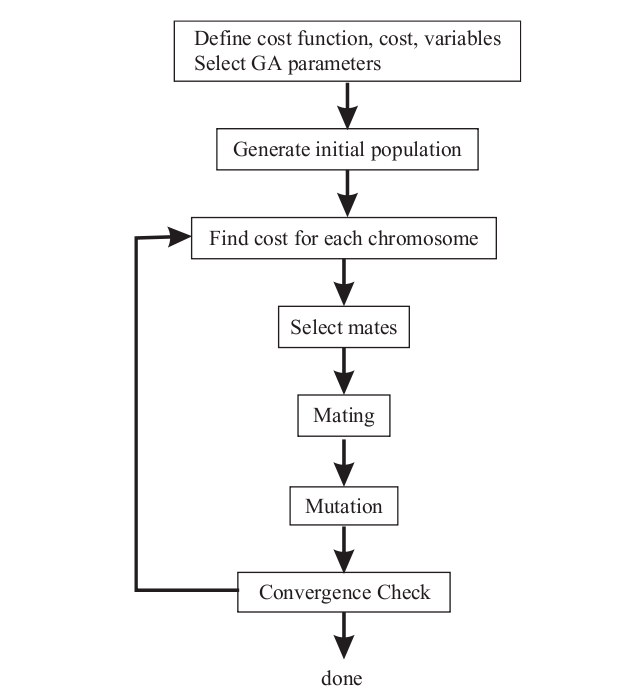
\includegraphics[scale=.4]{GA_flow.png}
  \end{center}
  \caption{GA flow chart \cite{Haupt:2004:PGA:1007746}}
\end{figure}

The GA operates on populations of chromosomes, successively changing one such population to another (by using GA operators: mutation, selection, crossover, etc.). 
Each chromosome contains potential solution to a problem (e.g. represented as binary string). 
Fitness functions are used to assess how well specific chromosome solves the problem.
The better fitting chromosomes are more likely to be involved in reproduction process.
That mimics the biological process of evolution - fitness of an organism is obtained by means of random variation (mutation, recombination, etc.) and natural selection
thus propagating genetic material to future generations.
These rules seems to be simple, but they are in fact responsible for extraordinary variety and complexity of the biosphere 
\cite{Mitchell01}. 
 
According to \cite{Mitchell01} , high parallelism, discovering and emphasizing solutions that are already quite good are the main reason why GAs work.  
 

\subsection{Genetic algorithms operators}

Following \cite{Mitchell01} - the simplest form of genetic algorithm involves three types of operators: selection, crossover and mutation. 

\begin{description}

\item[selection]
  This operator is responsible for selecting chromosomes from the population for reproduction.
  Likelihood of being chosen is based on the value of fitness function (the fitter the chromosome the better).
  
\item[crossover]
  The crossover operator is responsible for exchanging genetic material between chromosomes.
  Implemantation involves cutting points selection and then cut parts of chromosomes are exchanged.

\item[mutation]
  This operator introduces random changes to a chromosome.
  The probability of random change introduction is usually very small.  

\end{description}

\subsection{Application of EA to multi-objective optimization problems}

Evolutionary algorithms turn out to be very robust approach to multi-objective optimization problems.
Authors of \cite{drezewski2010review} tested their implementation on a set of well-known MOOPs \cite{drezewski2010review}:

\begin{itemize}
 \item Kursawe problem: \begin{equation} 
Kursawe \equiv
 \begin{cases}
       & f_{1}(x) = \sum_{i = 0}^{n - 1}(-10exp(-0.2\sqrt{(x_{i}^{2} + x_{i + 1}^2)})) \\
       &  f_{2}(x) = \sum_{i = 1}^{n}(|x_{i}|^{0.8} + 5 \sin({x_{i}^3}))  \\ 
			  &  n = 3,  -5 \leq x_{1}, x_{2}, x_{3} \leq 5 
			  
\end{cases}  
\end{equation}

  \item ZDT.
    
\end{itemize}

Results were compared with solutions proposed by one of the most popular multi-objective evolutionary algorithms that use elitism
 approach: NSGA-II and SPEA2 \cite{drezewski2010review}.

%---------------------------------------------------------------------------

\section{Co-evolutionary algorithms}
\label{sec:co-evol}

Co-evolutionary algorithms seem to have a huge advantage over evolutionary algorithms (EAs) - they can be applied to problems which do not have easily formulated 
fitness function (e.g. game-playing strategies).
It is commonly believed that they tend to perform better when dealing with infinite search spaces than regular EAs \cite{co-evol}.
Because of these advantages many researchers believe that they have a great potential.

Co-evolutionary algorithms rely on process of co-evolution (two or more species coexist and interact with each others in the same environment).
Individuals of one species interact with each other as well as with members of other species (which simulates the process of adaptation of different species cohabitating the same 
ecosystem).

The most widespread types of co-evolutionary algorithms include cooperative and competitive ones.
Cooperative algorithms tend to favour individuals working well with others.
Competetive methods are quite similar to the process of \emph{arm race} - minor adaptations in some individuals will force adjustment in others.
Because each subpopulation has to make changes in order to remain competetive, overall progress is guaranteed. 
  
It is possible that the population would seem to be changing but our fitness criteria may not register any improvement.
This could mean stagnation as well as arms race and is known as \emph{red queen effect} \cite{co-evol}.
In fact, this phenomena is a diagnostic problem because observing fitness measurements does not provide meaningful information about overall behaviour of the system.
 


Following \cite{Dre}, co-evolutionary interactions could include:

\begin{itemize}
  \item competition for limited resources;
  \item predator-prey interactions;
  \item host-parasite interactions;
  \item mutualism;
  \item commensalism.
\end{itemize}

The fitness of each individual simultaneously depends on fitness of the solution as well as other individuals' quality.
The biggest advantage of co-evolutionary algorithms is their ability to maintain population diversity which is crucial to obtain many good solutions in a single algorithm run.    

  
\subsection{Pseudocode of cooperative co-evolutionary algorithm}

According to \cite{co-evol}, the pseudocode of cooperative co-evolutionary algorithm is presented in Algorithm~\ref{pseudo_CEA}.

% \begin{algorithmic}
% 
% \FORALL{ population $p_s$ $\in$ $P$, all populations } 
% \STATE INITIALISE $p_s$
% \ENDFOR
% 
% \FORALL{ population $p_s$ $\in$ $P$, all populations } 
% \STATE EVALUATE $p_s$
% \ENDFOR
% 
% \STATE t := 0
% 
% \REPEAT
%   \FORALL{ population $p_s$ $\in$ $P$, all populations } 
%     \STATE SELECT parents from population $p_s$
%     \STATE GENERATE offspring from parents
%     \STATE SELECT collaborators $P$
%     \STATE EVALUATE offspring with collaborators
%     \STATE SELECT survivors for new population $P_s$
%   \ENDFOR  
%   \STATE t := t + 1
% \UNTIL{TERMINATING CRITERIA is met}
% 
% \end{algorithmic}

\begin{algorithm}
  \SetKwData{returnOrientedSubpopulation}{returnOrientedSubpopulation}
  \SetKwData{riskOrientedSubpopulation}{riskOrientedSubpopulation}
  \SetKwData{parents}{parents}
  \SetKwData{T}{T}
  \SetKwData{offspring}{offspring}
  \SetKwData{population}{population}
  \SetKwData{mutants}{mutants}
  \SetKwFunction{evaluate}{evaluate}
  \SetKwFunction{evaluateWithCollaborators}{evaluateWithCollaborators}
  \SetKwFunction{initialise}{initialise}
  \SetKwFunction{selectParents}{selectParents}
  \SetKwFunction{recombine}{recombine}
  \SetKwFunction{merge}{merge}
  \SetKwFunction{mutate}{mutate}
  \SetKwFunction{selectSurvivors}{selectSurvivors}
  \SetKwFunction{selectCollaborators}{selectCollaborators}

  \SetKwInOut{Input}{input}\SetKwInOut{Output}{output}
 

  \Input{a set of populations $P$}
  \BlankLine
  
  \ForEach{population $p_s$ $\in$ $P$}{
	  \initialise($p_s$)\;
  }

  \ForEach{population $p_s$ $\in$ $P$}{
	  \evaluate($p_s$)\;
   }

  \T $\leftarrow$ 0 \;

  \Repeat{TERMINATION CONDITION is satisfied}{
      \ForEach{population $p_s$ $\in$ $P$}{
	\parents $\leftarrow$  \selectParents{$p_s$} \;
	\offspring $\leftarrow$ \recombine{\parents} \;
	\selectCollaborators{$P$}
	\evaluateWithCollaborators{\offspring}  

	\ForEach{$individual$ $\in$ \offspring}{
	    \evaluate($individual$)\;
	}

	$p_s$ $\leftarrow$ \selectSurvivors{$p_s$} \;
      }
      \T $\leftarrow$ T + 1 \;
  }
  \caption{Pseudocode of generic CEA (\cite{co-evol})}\label{pseudo_CEA}
\end{algorithm}



A complete solution is formed by an individual combined with its collaborators.
 

\section{Multi-agent systems}
\label{sec:multi}

There is no universally accepted definition of the term \emph{agent}.
Nevertheless majority of researchers agree that \emph{agent} operates inside some \emph{environment} and should be capable of \emph{autonomous action}.
There is little agreement beyond this \cite{Weiss}. 
 
In theory it is possible to imagine a single agent working in an environment but it is quite rare.
The most common situation is a group of autonomous agents interacting inside the environment.
In order to be capable of fulfilling all the above requirements environments have to provide means of communications and interactions to all agents within.

\subsection{Intelligent agents}

The most useful type of \emph{agents} is called \emph{intelligent agent}.
The \emph{intelligent agent} is capable of \cite{Weiss}:

\begin{description}
  \item [Reactivity]
	  - agents can respond to changes in the environment and properly adjust to new conditions;
  \item [Pro-activeness]
	  - agents take the initiative to accomplish their goals;
  \item [Social ability]
	- agents are capable of intelligent interaction with other agents to satisfy their objectives.
\end{description}

\subsection{Co-evolutionary Multi-agent System (CoEMAS)}
\label{sec:CoEMAS}

According to  \cite{Dre} ,\cite{Dre2}, CoEMAS contains the following elements:

\begin{itemize}
  \item the environment; 
  \item the set of species that co-evolve; 
  \item the set of different resource types (there should be at least one resource type).
\end{itemize}

The environment contains information about available resources, its topography (usually represented as a weighted directed graph).
The species must coexist together, actions that any individual can perform depends on the nature of their coexistance.
In case od predator-prey model, prey individuals are capable of different actions than predators agents.


Additionally we define the set of actions that agent can perform :

\begin{description}
  \item [die]
      - agent dies when the amount of resources it helds is too low to sustain life (freed resource is given back to environment);
  \item [accept]
      - agent accepts partner for reproduction (only agents having more than threshold amount of resources are taken into account);
  \item [give]
      - agent is obliged to give some resource to other agent;
  \item [get]
      - agent is allowed to get some resource from other agent;
  \item [seek]
      - agent finds another agent so actions like get and finding appropriate partner for reproduction can be performed;
  \item [clone]
      - action of producing offspring - some amount of resources is passed to newly created agents from parents;
  \item [mutation]
      - this action is responsible for mutating the agent (introduces random genetic change);
  \item [migration]
      - agent is allowed to migrate from the current node to another;
  \item [recombination]
      - recombination operator is applied.

\end{description}


According to \cite{Dre}, the prey agent is allowed to perform one of the following operations : die, get, give, accept, seek, clone, recombination, mutation,
 migrate. Predator agent can perform seek, get, migrate actions.

Each agent has to realize its goals by following some predefined strategies.
Priority can be assigned to each strategy.
We can think of a strategy with a sheer goal of reproduction (only actions like seek, clone, recombination, mutation are allowed) or keeping individual alive
(actions like seek and get are performed).
After performing actions assigned to a particular strategy, a new strategy is elected. 

\subsection{Basic activities of agent in CoEMAS}

Pseudocode for activities of each agent is presented in Algorithm~\ref{pseudo_CoEMAS}.

\begin{algorithm}
  
  \SetKwData{Resource}{Resource}
  \SetKwData{profile}{profile}
  \SetKwData{InitialAmount}{InitialAmount}
  \SetKwFunction{chooseProfile}{chooseProfile}
  
  \SetKwInOut{Input}{input}\SetKwInOut{Output}{output}
 
  \BlankLine
  
  \tcc{assigning initial amount of resource to each agent}   
  \Resource $\leftarrow$  \InitialAmount \; 

  \tcc{agent tries to act according to one of the predefined profiles if its resource level allows it to live} 
  \While{\Resource > 0}{
      \tcc{choose a profile}
      \profile $\leftarrow$ \chooseProfile \;
      
      \If(){\profile is the $resource$ $profile$}{
	   \tcc{perform actions defined in $resource$ $profile$ which means obtaining more resources from other agents or environment} 
      }
      \ElseIf{\profile is the $reproduction$ $profile$}{
	    \tcc{perform actions defined in $reproduction$ $profile$ if amount of resource allows reproduction, 
			after reproduction the amount of resource possessed by an individual is lowered by a certain amount, which is given to offspring}
	}
      \ElseIf{\profile is the $migration$ $profile$}{ \tcc{perform actions defined in $migration$ $profile$ if amount of resource allows migration, some of the resource
	      held by an individual is passed to the environment (the migration process is not free)}}

     

  }
  \caption{Pseudocode of agent activities in CoEMAS }
  \label{pseudo_CoEMAS}
\end{algorithm}


It is obvious that applying these strategies we try to mimick behaviour of real organisms struggling in a hostile environment.

 
